\section{Pianificazione}
Si noterà che la pianificazione di Analisi dei requisiti è molto diversa, anche nella forma, dalle pianificazioni successive. Ciò è dovuto ai cambiamenti apportati al nostro modello di sviluppo e pianificazione. Abbiamo ritenuto comunque di lasciare la pianificazione della fase di Analisi dei requisiti, visto che quel periodo è stato effettivamente svolto usandola come riferimento.


Lo sviluppo del progetto è diviso nei seguenti periodi:
\begin{enumerate}
	\item Analisi dei requisiti;
	\item Progettazione architetturale;
	\item Progettazione di dettaglio e codifica;
	\item Validazione e collaudo.
\end{enumerate} 

\subsection{Analisi dei requisiti (dal 2020-10-22 al 2021-01-17)}

\subsubsection{Ruoli attivi}
\begin{itemize}
	\item Responsabile;
	\item Amministratore;
	\item Analista;
	\item Verificatore.
\end{itemize}

\subsubsection{Periodi e attività}

\paragraph{Primo periodo (dal 2020-10-22 al 2020-11-09)}
Questo periodo comincia con la costituzione del gruppo di progetto. Serve dunque a porre le basi per una comunicazione e collaborazione efficace ed efficiente. Vi si svolgono inoltre attività di ricerca superficiale sui capitolati.

\begin{itemize}
	\item Configurazione degli strumenti collaborativi basilari: comprende la scelta e la configurazione dei mezzi per la comunicazione e il lavoro collaborativo;
	\item Analisi superficiale dei capitolati.
	
\end{itemize}

\paragraph{Secondo Periodo (dal 2020-11-10 al 2020-12-13)}
Gli obiettivi raggiunti in questo periodo sono il consolidamento degli strumenti di collaborazione e l'approfondimento dei capitolati.
\begin{itemize}
	\item Configurazione del \glock{repository}: questa attività comprende la creazione di un repository per la condivisione e il versionamento dei prodotti, ma anche la sua configurazione per la verifica automatica della loro validità;
	\item Raccolta di informazioni dai seminari: stesura di appunti sui seminari, da poter facilmente consultare quando necessario;
	\item Studio dei progetti degli anni passati: questa attività ha il fine di individuare gli errori più comuni e le tecniche da prendere come esempio;
	\item Bozza dello studio di fattibilità;
	\item Bozza delle norme di progetto.
\end{itemize}

\paragraph{Terzo Periodo (dal 2020-12-14 al 2020-01-08)}
Questo periodo segue la scelta del capitolato da affrontare. È dedicato alla sua analisi approfondita e alla stesura della documentazione. 
\begin{itemize}
	\item Stesura delle norme di progetto;
	\item Stesura dello studio di fattibilità;
	\item Stesura del piano di progetto;
	\item Analisi dei requisiti e stesura dell'omonimo documento;
	\item Stesura del piano di qualifica;
	\item Stesura del glossario;
	\item Stesura della lettera di presentazione;
	\item Aggiornamento consuntivo;
	\item Verifica della documentazione.
\end{itemize}

\paragraph{Quarto Periodo (dal 2020-01-09 al 2020-01-17)}
È l'ultimo periodo di analisi dei requisiti. Si concentra quindi sulla preparazione dell'esposizione dei prodotti dei tre periodi precedenti.
\begin{itemize}
	\item Preparazione dell'esposizione;
	\item Verifica dell'esposizione.
\end{itemize}


\begin{landscape}
	\begin{figure}[H]
		\centering
		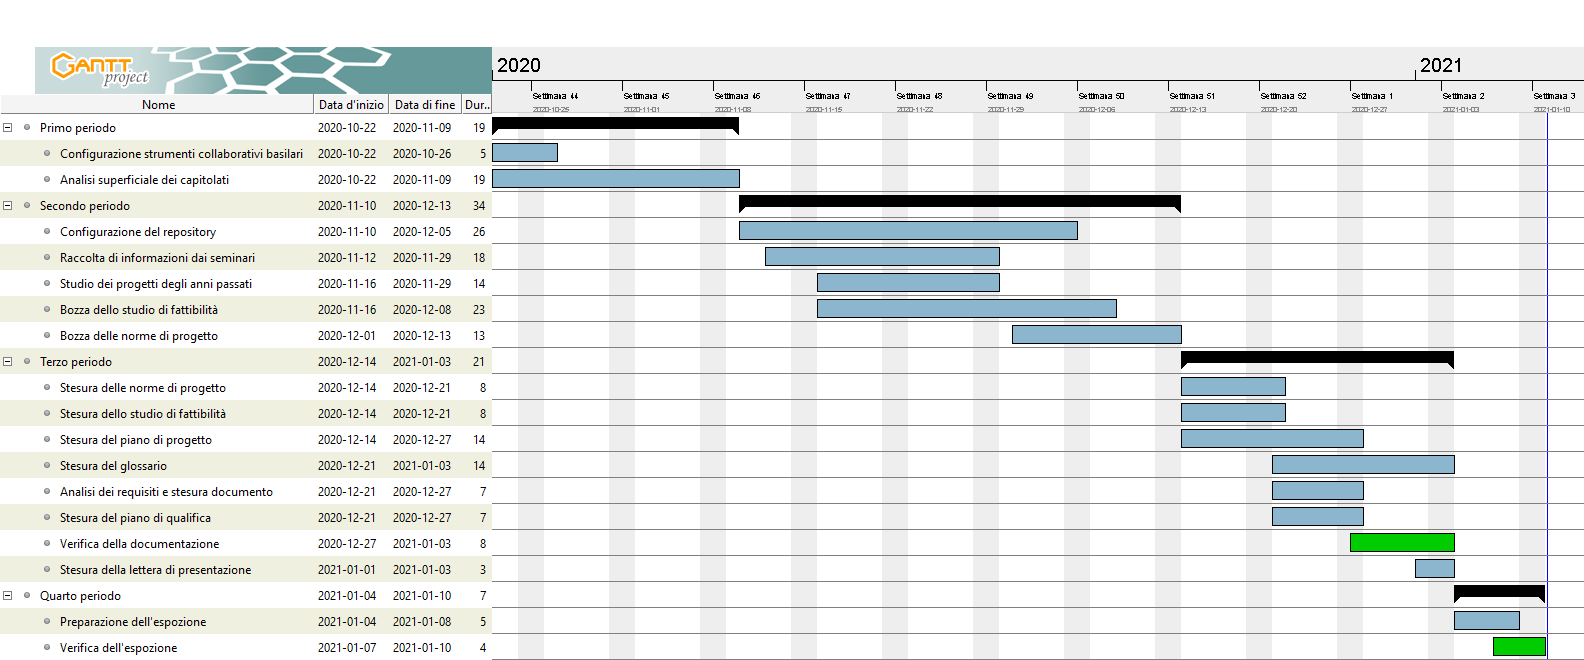
\includegraphics[width=\linewidth]{res/images/ganttFase1.png}
		\caption*{\textbf{Figura 1}{: Grafico di Gantt del periodo di analisi dei requisiti}}
		\label{fig:Gantt Analisi dei requisiti}
	\end{figure}
\end{landscape}



\noindent Di seguito vengono riportare le attività che si é previsto di svolgere durante i macroperiodi rimanenti. Per ogni attività e per ogni ruolo viene indicata una quantità di ore che si prevede saranno necessarie per svolgerla. Alcune celle ricoprono più righe. In quei casi la somma delle ore richieste dall'insieme di attività per quel ruolo è pari al valore della cella. Si è deciso di accorpare più celle per evitare valori frazionari. \newline
\indent Le ore sono state distribuite prendendo come riferimento il preventivo del punto §4 e apportandovi modifiche basate sul Preventivo a finire del documento Piano di Progetto v. 1.0.0. A partire dall'attuale versione del documento (Piano di Progetto v. 1.0.0) si è deciso di redigere un Preventivo a finire che mostri una pianificazione per i periodi successivi. Così facendo, il contenuto del Preventivo a finire di questa versione potrà essere utilizzato come Pianificazione nella versione successiva. \newline
\indent La distribuzione delle ore riguarda tutti i periodi rimanenti, tuttavia più la previsione è lontana nel futuro, più la sua realizzazione è difficile. Abbiamo deciso di redigere comunque una pianificazione per i periodi più lontani in modo da applicarvi i miglioramenti dedotti, ad ogni versione, dai periodi precedenti. \newline

\subsection{Progettazione architetturale (dal 2021-01-18 al 2021-03-07)}

Questo periodo porta alla milestone della Revisione di Progettazione.
Durante questo periodo si vogliono individuare le tecnologie da utilizzare per lo sviluppo del prodotto e l'architettura su cui basarlo.


\subsubsection{Pianificazione di macroperiodo}
\begin{table}[H]
	\rowcolors{2}{lightest-grayest}{white}
	\centering
	\renewcommand{\arraystretch}{1.5}
	\begin{tabular}{|c|p{10mm}|p{10mm}|p{10mm}|p{10mm}|p{10mm}|p{10mm}|}
		\hline
		\rowcolor{lighter-grayer}
		Attività & Re & Am & An & Pt & Pm & Ve \\ \hline
		Aggiornamento PdQ & \cellcolor{white}  & - &  & - & - & 20 \\
		Aggiornamento Adr & \cellcolor{white} & - & 40 & - & - & 2 \\
		Aggiornamento NdP & \multirow{-3}*{\cellcolor{white}2} & 6 & - & - & - & 2 \\ \hline
		Aggiornamento PdP     & 10	& - & - & - & - & 2  \\ \hline
		Technology baseline   & 1	& -  & - & 20 & - & -   \\ \hline
		Proof of concept      & 1	& - & - & 40 & - & -   \\ \hline
		Attività accessorie   & 2& 5 & 1  & 2  &  & 4  \\ \hline
		Comunicazione con docenti               & 2& - & - & - & - & -   \\ \hline
		Comunicazione con proponente            & 2& - & - & - & - & -   \\ \hline
		Presentazione         & 1& 1 & 1  & 1  &  & 1 \\
		\hline
	\end{tabular}
	\caption*{\textbf{Tabella 1}: Pianificazione riguardante il periodo di Progettazione architetturale\\}
\end{table}

\subsubsection{Pianificazione di microperiodo}
\indent La pianificazione settimanale che segue riporta la suddivisione oraria tra i ruoli ma non tra i componenti. Si è deciso di escludere questa informazione dal documento, anche se essa è presente nello strumento utilizzato, per rendere la lettura più semplice.

\paragraph{Microperiodo 1}
\begin{table}[H]
	\rowcolors{2}{lightest-grayest}{white}
	\centering
	\renewcommand{\arraystretch}{1.5}
	\begin{tabular}{|c|p{10mm}|p{10mm}|p{10mm}|p{10mm}|p{10mm}|p{10mm}|}
		\hline
		\rowcolor{lighter-grayer}
		Attività & Re & Am & An & Pt & Pm & Ve \\ \hline
		Aggiornamento PdQ & \cellcolor{white} & \cellcolor{white} & \cellcolor{white} & \cellcolor{white} & \cellcolor{white} & \cellcolor{white} \\
		Aggiornamento AdR & \cellcolor{white} & \cellcolor{white} & \cellcolor{white} & \cellcolor{white} & \cellcolor{white} & \cellcolor{white} \\
		Aggiornamento NdP & \cellcolor{white} & \cellcolor{white} & \cellcolor{white} & \cellcolor{white} & \cellcolor{white} & \cellcolor{white} \\
		Aggiornamento PdP & \multirow{-4}*{\cellcolor{white}2} & \multirow{-4}*{\cellcolor{white}1} & \multirow{-4}*{\cellcolor{white}8} & \multirow{-4}*{\cellcolor{white}-} & \multirow{-4}*{\cellcolor{white}-} & \multirow{-4}*{\cellcolor{white}5} \\
		\hline
	\end{tabular}
	\caption*{\textbf{Tabella 1}: Pianificazione riguardante il periodo di Progettazione architetturale\\}
\end{table}


\paragraph{Microperiodo 2}
\begin{table}[H]
	\rowcolors{2}{lightest-grayest}{white}
	\centering
	\renewcommand{\arraystretch}{1.5}
	\begin{tabular}{|c|p{10mm}|p{10mm}|p{10mm}|p{10mm}|p{10mm}|p{10mm}|}
		\hline
		\rowcolor{lighter-grayer}
		Attività & Re & Am & An & Pt & Pm & Ve \\ \hline
		Aggiornamento PdQ & \cellcolor{white} & \cellcolor{white} & \cellcolor{white} & \cellcolor{white} & \cellcolor{white} & \cellcolor{white} \\
		Aggiornamento AdR & \cellcolor{white} & \cellcolor{white} & \cellcolor{white} & \cellcolor{white} & \cellcolor{white} & \cellcolor{white} \\
		Aggiornamento NdP & \cellcolor{white} & \cellcolor{white} & \cellcolor{white} & \cellcolor{white} & \cellcolor{white} & \cellcolor{white} \\
		Aggiornamento PdP & \multirow{-4}*{\cellcolor{white}2} & \multirow{-4}*{\cellcolor{white}1} & \multirow{-4}*{\cellcolor{white}8} & \multirow{-4}*{\cellcolor{white}-} & \multirow{-4}*{\cellcolor{white}-} & \multirow{-4}*{\cellcolor{white}5} \\
		\hline
		Technology baseline & - & - & - & 20 & - & - \\
		\hline
	\end{tabular}
	\caption*{\textbf{Tabella 1}: Pianificazione riguardante il periodo di Progettazione architetturale\\}
\end{table}

\paragraph{Microperiodo 3}
\begin{table}[H]
	\rowcolors{2}{lightest-grayest}{white}
	\centering
	\renewcommand{\arraystretch}{1.5}
	\begin{tabular}{|c|p{10mm}|p{10mm}|p{10mm}|p{10mm}|p{10mm}|p{10mm}|}
		\hline
		\rowcolor{lighter-grayer}
		Attività & Re & Am & An & Pt & Pm & Ve \\ \hline
		Aggiornamento PdQ & \cellcolor{white} & \cellcolor{white} & \cellcolor{white} & \cellcolor{white} & \cellcolor{white} & \cellcolor{white} \\
		Aggiornamento AdR & \cellcolor{white} & \cellcolor{white} & \cellcolor{white} & \cellcolor{white} & \cellcolor{white} & \cellcolor{white} \\
		Aggiornamento NdP & \cellcolor{white} & \cellcolor{white} & \cellcolor{white} & \cellcolor{white} & \cellcolor{white} & \cellcolor{white} \\
		Aggiornamento PdP & \multirow{-4}*{\cellcolor{white}2} & \multirow{-4}*{\cellcolor{white}1} & \multirow{-4}*{\cellcolor{white}8} & \multirow{-4}*{\cellcolor{white}-} & \multirow{-4}*{\cellcolor{white}-} & \multirow{-4}*{\cellcolor{white}5} \\
		\hline
		Comunicazione con docenti & 1 & - & - & - & - & - \\
		\hline
		Proof of Concept & - & - & - & 20 & - & - \\
		\hline
	\end{tabular}
	\caption*{\textbf{Tabella 1}: Pianificazione riguardante il periodo di Progettazione architetturale\\}
\end{table}

\paragraph{Microperiodo 4}
\begin{table}[H]
	\rowcolors{2}{lightest-grayest}{white}
	\centering
	\renewcommand{\arraystretch}{1.5}
	\begin{tabular}{|c|p{10mm}|p{10mm}|p{10mm}|p{10mm}|p{10mm}|p{10mm}|}
		\hline
		\rowcolor{lighter-grayer}
		Attività & Re & Am & An & Pt & Pm & Ve \\ \hline
		Aggiornamento PdQ & \cellcolor{white} & \cellcolor{white} & \cellcolor{white} & \cellcolor{white} & \cellcolor{white} & \cellcolor{white} \\
		Aggiornamento AdR & \cellcolor{white} & \cellcolor{white} & \cellcolor{white} & \cellcolor{white} & \cellcolor{white} & \cellcolor{white} \\
		Aggiornamento NdP & \cellcolor{white} & \cellcolor{white} & \cellcolor{white} & \cellcolor{white} & \cellcolor{white} & \cellcolor{white} \\
		Aggiornamento PdP & \multirow{-4}*{\cellcolor{white}3} & \multirow{-4}*{\cellcolor{white}1} & \multirow{-4}*{\cellcolor{white}8} & \multirow{-4}*{\cellcolor{white}-} & \multirow{-4}*{\cellcolor{white}-} & \multirow{-4}*{\cellcolor{white}5} \\
		\hline
		Proof of Concept & - & - & - & 20 & - & - \\
		\hline
	\end{tabular}
	\caption*{\textbf{Tabella 1}: Pianificazione riguardante il periodo di Progettazione architetturale\\}
\end{table}


\paragraph{Microperiodo 5}
\begin{table}[H]
	\rowcolors{2}{lightest-grayest}{white}
	\centering
	\renewcommand{\arraystretch}{1.5}
	\begin{tabular}{|c|p{10mm}|p{10mm}|p{10mm}|p{10mm}|p{10mm}|p{10mm}|}
		\hline
		\rowcolor{lighter-grayer}
		Attività & Re & Am & An & Pt & Pm & Ve \\ \hline
		Aggiornamento PdQ & \cellcolor{white} & \cellcolor{white} & \cellcolor{white} & \cellcolor{white} & \cellcolor{white} & \cellcolor{white} \\
		Aggiornamento AdR & \cellcolor{white} & \cellcolor{white} & \cellcolor{white} & \cellcolor{white} & \cellcolor{white} & \cellcolor{white} \\
		Aggiornamento NdP & \cellcolor{white} & \cellcolor{white} & \cellcolor{white} & \cellcolor{white} & \cellcolor{white} & \cellcolor{white} \\
		Aggiornamento PdP & \multirow{-4}*{\cellcolor{white}3} & \multirow{-4}*{\cellcolor{white}2} & \multirow{-4}*{\cellcolor{white}8} & \multirow{-4}*{\cellcolor{white}-} & \multirow{-4}*{\cellcolor{white}-} & \multirow{-4}*{\cellcolor{white}6} \\
		\hline
		Presentazione & 1 & 1 & 1 & 1 & - & 1 \\
		\hline
		Attività accessorie & 2 & 5 & 1 & 2 & - & 4 \\
		\hline
	\end{tabular}
	\caption*{\textbf{Tabella 1}: Pianificazione riguardante il periodo di Progettazione architetturale\\}
\end{table}


\subsection{Progettazione di dettaglio e codifica (dal 2021-03-08 al 2021-04-08)}


\subsubsection{Attività da svolgere e distribuzione delle ore prevista}
\begin{table}[H]
	\rowcolors{2}{lightest-grayest}{white}
	\centering
	\renewcommand{\arraystretch}{1.5}
	\begin{tabular}{|c|p{10mm}|p{10mm}|p{10mm}|p{10mm}|p{10mm}|p{10mm}|}
		\hline
		\rowcolor{lighter-grayer}
		Attività & Re & Am & An & Pt & Pm & Ve \\ \hline
		Aggiornamento PdQ& 1 & - & - & - & - & 20 \\ \hline
		Aggiornamento AdR& 1 & - & 20 & - & - & 2  \\ \hline
		Aggiornamento NdP& 1 & 10 & - & - & - & 2  \\ \hline
		Aggiornamento PdP& 10& - & - & - & - & 2  \\ \hline
		Product baseline & 2 & - & - & 18 & - & 2  \\ \hline
		Codifica della struttura delle componenti     & 2 & - & - & - & 35 & 15 \\ \hline
		\begin{tabular}[x]{@{}c@{}}Codifica delle interazioni \\ tra le componenti interne\end{tabular}      & 2 & - & - & - & 35 & 15 \\ \hline
		Codifica delle interazioni con gli attori esterni  & 2 & - & - & - & 35 & 15 \\ \hline
		\begin{tabular}[x]{@{}c@{}}Codifica delle funzionalità secondarie \\ non ancora implementate\end{tabular} & 1 & - & - & - & 32 & 15 \\ \hline
		Stesura manuale utente& \cellcolor{white}  & 12 & - & - & - & 4  \\
		Stesura manuale manutentore & \multirow{-2}*{\cellcolor{white}1}  & 12 & - & - & - & 4  \\ \hline
		Attività accessorie    & 2 & 5  & 1  & 1  & 2  & 3  \\ \hline
		Comunicazione con docenti   & 2 & - & - & - & - & -   \\ \hline
		Comunicazione con proponente& 2 & - & - & - & - & -   \\ \hline
		Presentazione    & 1 & 1  & 1  & 1  & 1  & 1 \\
		\hline
	\end{tabular}
	\caption*{\textbf{Tabella 2}: Pianificazione riguardante il periodo di Progettazione di dettaglio e codifica\\}
\end{table}


\subsection{Validazione e collaudo (dal 2021-04-09 al 2021-05-09)}


\subsubsection{Attività da svolgere e distribuzione delle ore prevista}
\begin{table}[H]
	\rowcolors{2}{lightest-grayest}{white}
	\centering
	\renewcommand{\arraystretch}{1.5}
	\begin{tabular}{|c|p{10mm}|p{10mm}|p{10mm}|p{10mm}|p{10mm}|p{10mm}|}
		\hline
		\rowcolor{lighter-grayer}
		Attività & Re & Am & An & Pt & Pm & Ve \\ \hline
		Aggiornamento PdQ          & 1  & 10 & - & - & - & 10 \\ \hline
		Aggiornamento NdP          & 1  & 10 & - & - & - & 5  \\ \hline
		Aggiornamento PdP          & 10 & - & - & - & - & 4  \\ \hline
		Validazione                & 2  & - & - & 12 & 21 & 20 \\ \hline
		Collaudo                   & 2  & - & - & 11 & 20 & 20 \\ \hline
		Attività accessorie 	   & 2  & 7  & - & 1  & 1  & 3  \\ \hline
		Comunicazione con docenti  & 2  & - & - & - & - & -   \\ \hline
		Comunicazione con proponente& 2  & - & - & - & - & -   \\ \hline
		Presentazione              & 1  & 1  & - & 1  & 1  & 1 \\
		\hline
	\end{tabular}
	\caption*{\textbf{Tabella 3}: Pianificazione riguardante il periodo di Validazione e collaudo\\}
\end{table}